\chapter{Check of the assumptions}
For the whole workflow several assumptions about the data or the results of certain transformations are made. These assumptions have to be met at least roughly to ensure the correctness of the results.\newline
This section gives checks for most of the assumptions like accuracy of the PSF scale estimation or that the matched filter of the matching size compared to the PSF performs best.
\section{Calibration measurement}
As described by \cite{meanVar} the gain can be determined using the mean and variance of data with different mean intensities. Therefore a calibration dataset was aquired. The temperature and the gain factor were set to match the settings usually used. A sample with cells was prepared for the Storm measurement. First, eleven time series were taken, with opend shutter and with increasing exposure time from 0 milliseconds up to 1000 milliseconds. Afterwards the same procedure was repeated with the shutter kept closed. Figure \ref{calibplot} shows the results for the first 6 exposure time. All points lie on a straight line. The gain factor determined by the calibration measurement was 3.9, the offset 315. This offset is too small. An other methode was used to determine the offset. There were also an other series of  images taken with closed shutter. This series shows the response of the camera without any light around. The mean value of the shortest exposure time was taken as offset. Its value is 380. 
\begin{figure}
\centering
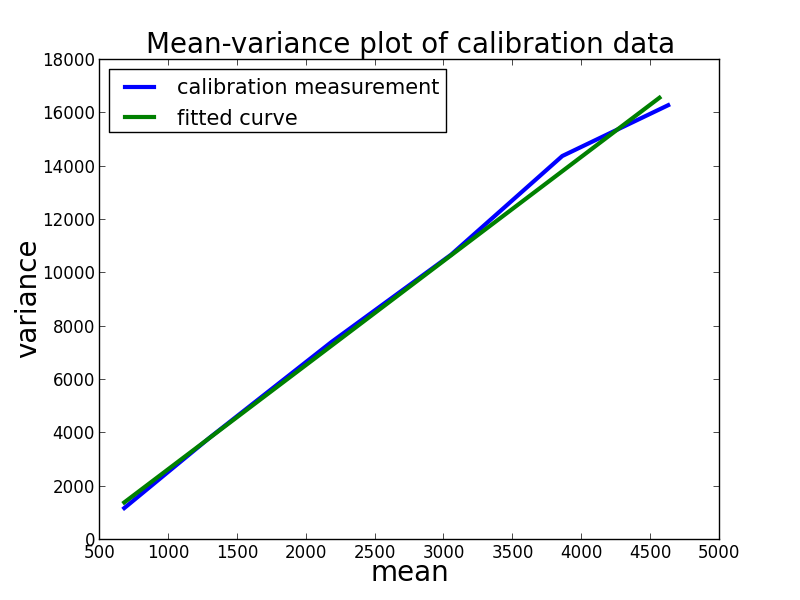
\includegraphics[width = 0.88\textwidth]{pictures/meanVariancePlotCalibration.png}
	 \caption{Result of the calibration measurements. The gain determined from this variance-mean plot is 3.9.}
	\label{calibplot}
\end{figure}


\section{Correction to Poisson distributions}
It is very important for the whole workflow that the first transform results in background intensities that follow a Poisson distribution. To test this, a real world image was transformed with parameters taken from the calibration measurement described in the previous section. The offset was estimated from the minimal intensity of the raw image. The histograms for two generic background pixels are shown in Figure \ref{isitPoisson}. A Poisson distribution with the mean of the pixels intensities is also shown in the figures. These histograms were aquired using the pixel intensities of one pixel for 3000 frames. The histogram matches the expected Poisson distribution.
\begin{figure}
\subfloat[Tubulin2 frame 10]{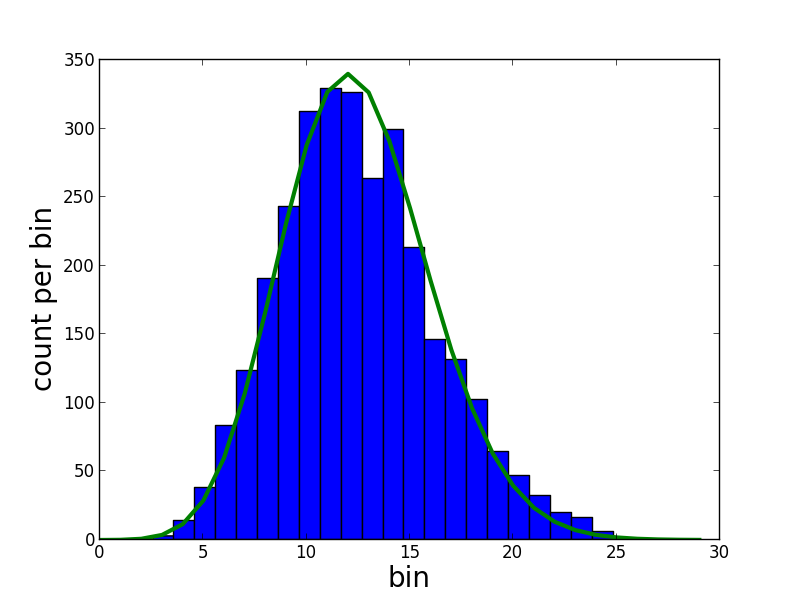
\includegraphics[width = 0.485\textwidth]{pictures/IsItPoisson105_105.png}}\hfill
\subfloat[Tubulin2 frame 1010]{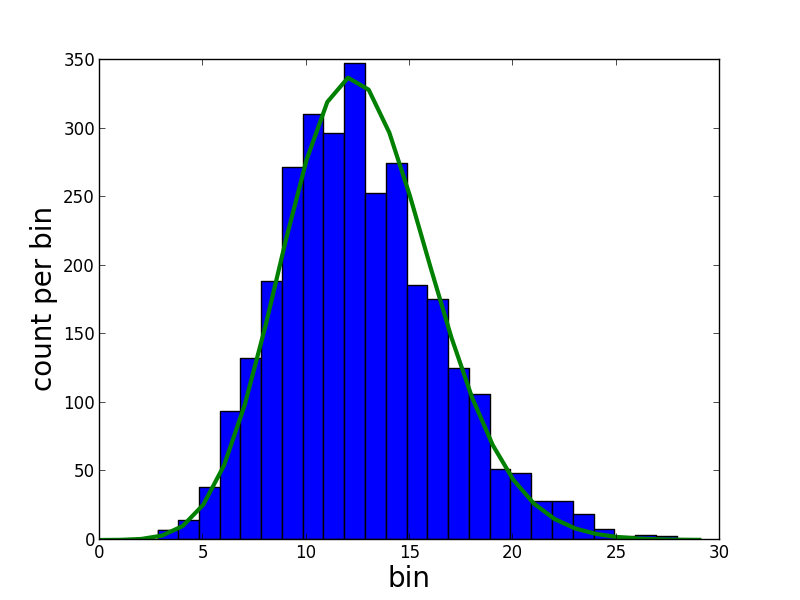
\includegraphics[width = 0.485\textwidth]{pictures/IsItPoisson50_50.png}}
	\caption{These pictures show how well the histograms of background pixels taken over the first 3000 frames, follow a Poisson distribution. For the gain the parameter from the calibration measurement of $g$ = 3.9 was used. The offset was estimated from the minimal intensities of the original image.}
	\label{isitPoisson}	
\end{figure}

\section{Result Anscombe transformation}
After the transformation described in \ref{trafoPoiss}, the Anscombe transformation was aplied on the same data set that was used in the previous section and the background was subtracted. Figure \ref{isitAnscombe} shows the histogram of the intensities of one randomly chosen frame and a Gaussian with zero mean and unit variance. The histogram fits very well to the Gaussian. The tail exceeding the Gaussian on the right side can at least partially be explained by the signal that is present in the image and does not follow the Gaussian distribution, but has higher intensities.
\begin{figure}
\centering
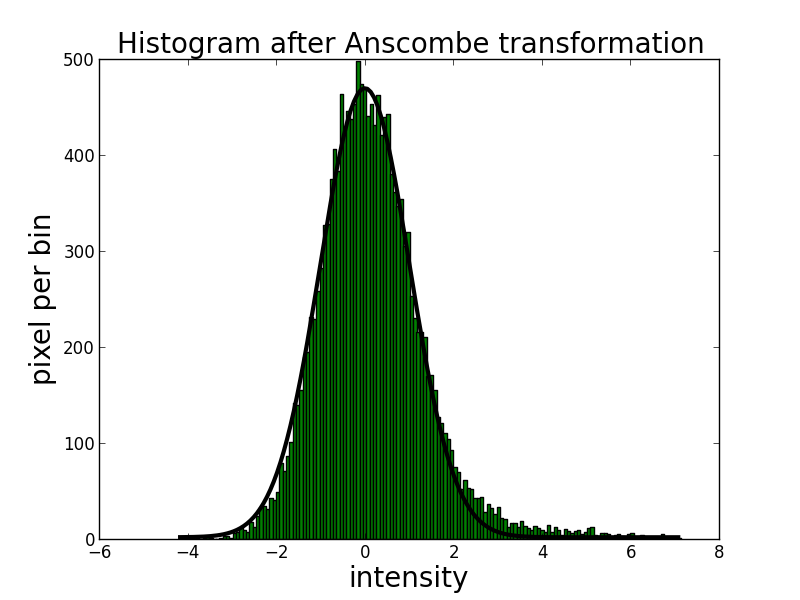
\includegraphics[width = 0.88\textwidth]{pictures/anscombeAndFit.png}
	 \caption{After the Anscombe transformation the background pixel intensities should be distributed with mean zero and variance one. This figure shows the histogram of the pixel intensities and a fitted Gaussian with variance one and mean zero.}
	\label{isitAnscombe}
\end{figure}

\section{Accuracy of detection}
Unfortunately the position of the flourescent molecules can not be detected
perfectly. There are two main contribution to the errors in detection.\\
On one hand, there is a problem with finding the maximum in a noisy signal. Due to
noise the spots maxima might be shifted.\newline
On the other hand, the position of the fluorescent molecule is deteted by upscaling the pixel grid and interpolation.
After that the maximums position of the upscaled grid is taken as the resulting
position. This gives an error from roughly a 12th pixelwidth. This error becomes less important with higher upscaling factors.\newline

Because there is no groundtruth for the real data, we had to produce test data and groundtruth. This was done similar to the method described by \cite{simulated}. The difference was, that instead of generating just one spot per frame a different number of spots were simulated for each frame. For different signal-to -noise ratios, a dataset with 40 times 40 pixels and 1000 frames was created. Each frame containing one, three or five point spread functions. The position of the spots was determined beforehand, to use the same spots for each signal to noise ratio.\newline

To determine the accuracy, the standard deviation between the true position of the signal and its detection were used. For data sets with more than one spot per frame, the best match within a certain distance around the true position was found. If a pair of true spot and detection were found, both were removed for further matching of the remaining signals. In the end the averaged standard deviation of the detection relative to the true positions were calculated as follows:
\begin{align}
	\text{std. dev.} = \sum_i \sqrt{\left(\bf{p}_{\text{true}}^i - \bf{p}_{\text{detec}}^i\right)^2}
\end{align}
$i$ runs over all found pairs of groundtruth and detections, $\bf{p}$ describes the two dimensional spatial vector of the groundtruth or detection respectivly.\newline

The results can be seen in Figure \ref{accplot}. The Figure shows, that the more spots are present per frame the harder it is to detect them properly. This is a result of the fact that spots that lay near each other might be detected as one spot. This gives rise to higher errors in the detection accuracy.


\begin{figure}
\begin{minipage}[t]{0.48\textwidth}
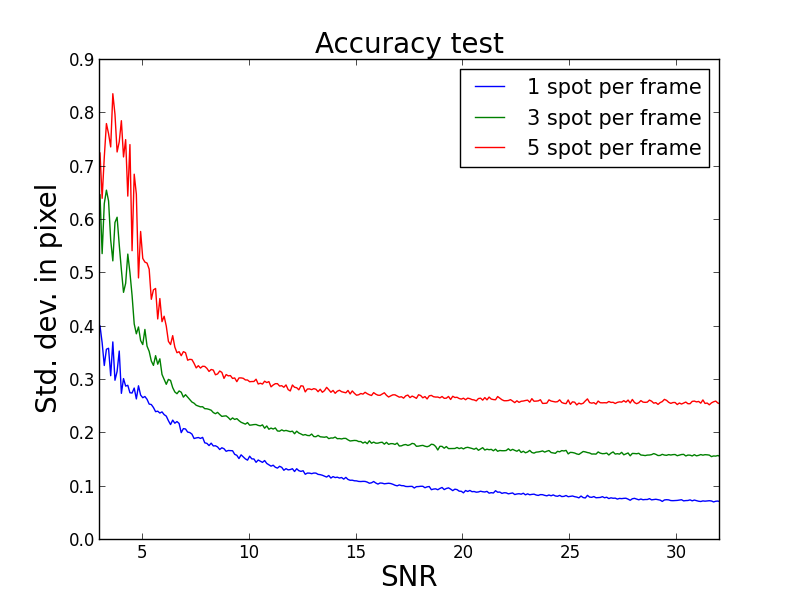
\includegraphics[width = 0.99\textwidth]{pictures/AccuracyTest.png}
	\caption{Result of the accuracy test. For datasets with one, three or five point spread functions per frame, evaluated for different signal to noise levels. The more dense the spots are the less accurate the detections are.}
	\label{accplot}	
\end{minipage}\hfill
\begin{minipage}[t]{0.48\textwidth}
\centering
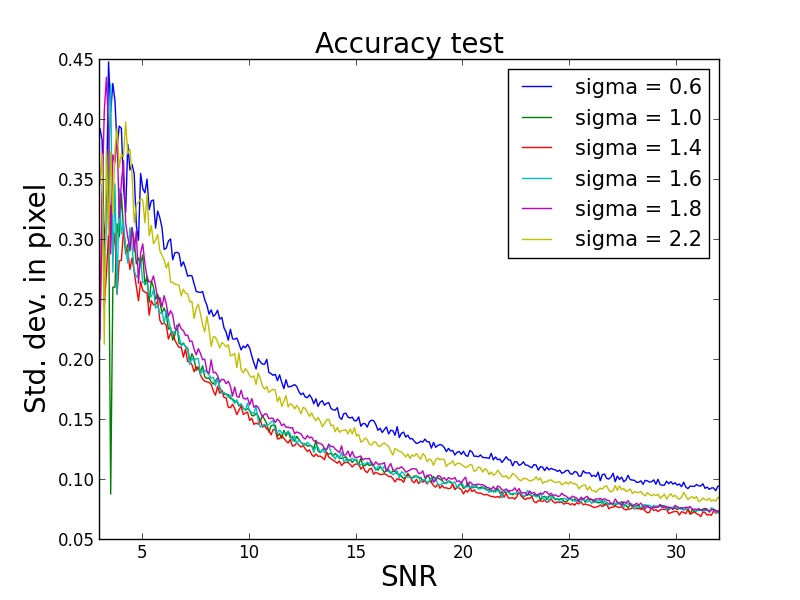
\includegraphics[width = 0.99\textwidth]{pictures/AccuracyTestSigma.png}
	\caption{Result of the accuracy test for different sigmas for the Gaussian smoothing. One data set was processed with different sigma values and evaluated for different signal to noise levels. The true standard deviation of point spread function of the simulated data is 1.4.}
	\label{accplot2}

\end{minipage}
\end{figure}


\section{Matched filter is best filter} \label{detectionError}
For denoising the image a matched filter is used. Since we assume that the point spread function is Gaussian, a two dimensional Gaussian filter with the estimated size of the point spread function is used. The following calculation shows why this is the best choice for the standard deviation.\newline
This calculation was inspired by the calculation in \cite{ulli}.\newline 
The assumptions are, the point spread function is Gaussian shaped with a true standard deviation of $\sigma_\text{PSF}$, the image contains white Gaussian noise with mean zero and unit variance, the applied filter for denoising is a Gaussian filter with standard deviation $\sigma_\text{filter}$.\newline
The image $f$ is composed of Gaussian filter convolved with the signal $s$ and the above mentioned white noise $n$. $s$ and $n$ describe the filtered signal respectivly noise.
\begin{align}
 f=s+n \label{gl91}
\end{align}
Without noise the first derivative of $f$ which is equal to $s$ in the noise-free case vanishs at the center of the Gaussian signal. This center can be set to the origin without losing generality. But noise shifts the zero crossing of the first derivatives to $\Delta x,~\Delta y$. For now just one dimension is considered.
\begin{align}
\frac{\partial f}{\partial x}\left(\Delta x, \Delta y\right) &= \frac{\partial s}{\partial x} \left(\Delta x, \Delta y\right) + \frac{\partial n}{\partial x}\left(\Delta x, \Delta y\right)&=0
\end{align}  

Using Taylor expansion around $x = 0$ at $y= 0$ for the signal, yields:
\begin{align}
f_x(\Delta x, \Delta y)&\approx \underbrace{s_x(0, 0)}_{=0} + s_{xx}(0, 0)\cdot \Delta x + n_x(\Delta x, \Delta y)&=0\\
\Rightarrow \text{var}(s_{xx}(0, 0)\cdot \Delta x)&= \text{var}(n_x(\Delta x,\Delta y)\\
\Rightarrow \text{var}(\Delta x) &= \frac{\text{var}(n_x(\Delta x, \Delta y)}{s_{xx}^2(0, 0)} \label{ch9gl1}
\end{align}

The result for the variance of the first derivative of white noise convolved with a Gaussian filter of width $\sigma_\text{filter}$ can be found at \cite{ulli}. It is:
\begin{align}
	\text{var}(n_x) = \frac{N^2}{8\pi\sigma_\text{filter}^4},~\text{with }N\text{: noise std. dev} \label{ch9gl2}
\end{align}
The convolution of the Gaussian PSF  with an other Gaussian results in Gaussian with combined scales.
\begin{align}
 \mathcal{N}(0,\sigma_\text{PSF}) \ast \mathcal{N}(0,\sigma_\text{filter}) = \mathcal{N}\left(0,\underbrace{\sqrt{\sigma_\text{PSF}^2+\sigma_\text{filter}^2}}_{=\sigma_\text{comb}}\right)
\end{align}
The value of the second derivative in $x$-direction of the convolved PSF at (0,0) is:
\begin{align}
 \frac{\partial^2 S_0\cdot\mathcal{N}\left((\mu_x,\mu_y),\sigma_\text{comb}\right)}{\partial x^2}  &=  -\frac{S_0}{2\pi \sigma_\text{comb}^4}  \label{ch9gl3}
\end{align}
Combining \ref{ch9gl1}, \ref{ch9gl2} and \ref{ch9gl3} yields:
\begin{align}
\text{var}\left(\Delta x\right) &= \dfrac{\dfrac{N^2}{8\pi\sigma_\text{filter}^4}}{\dfrac{S_0^2}{4\pi^2 \sigma_\text{comb}^8}}\\
&= \frac{N^2\cdot 4\pi^2 \sigma_\text{comb}^8}{S_0^2\cdot8\pi\sigma_\text{filter}^4}\\
&= \frac{N^2}{S_0^2} \frac{\pi \left(\sigma_\text{filter}^2+\sigma_\text{PSF}^2\right)^4}{2\sigma_\text{filter}^4}\\
&= \frac{N^2\pi}{2S_0^2} \left(1+\frac{\sigma_\text{PSF}^2}{\sigma_\text{filter}^2}\right)^2\left(\sigma_\text{filter}^2+\sigma_\text{PSF}^2\right)^2 
\end{align}
The same calculation can be done with respect to $y$. This gives the same variance, yielding a total variance that is square root of 2 times larger, because the variances are orthogonal.
Therefore the standard deviation of the localization is:
\begin{align}
 \text{std. dev loc}&=\frac{N}{S_0}\sqrt{\frac{\sqrt{2}\pi}{2}}
 \left(1+\frac{\sigma_\text{PSF}^2}{\sigma_\text{filter}^2}\right)\left(\sigma_\text{filter}^2+\sigma_\text{PSF}^2\right) 
\end{align}
To verify these results test data sets have been created containing 3500 frames with one PSF per frame. Each created data set contained a PSF with different scale. This data sets have been filtered with Gaussian filters of different sizes. After that the maximum for each frame was detected and compared with the true position. Figure \ref{matchedFilter1} shows the accuracy for different PSF scales and filter widths.\newline
The best results were achieved using a Gaussian filter with the PSFs size. The larger the PSFs scale the more inaccurate the localization becomes.\newline

\begin{figure}
\centering
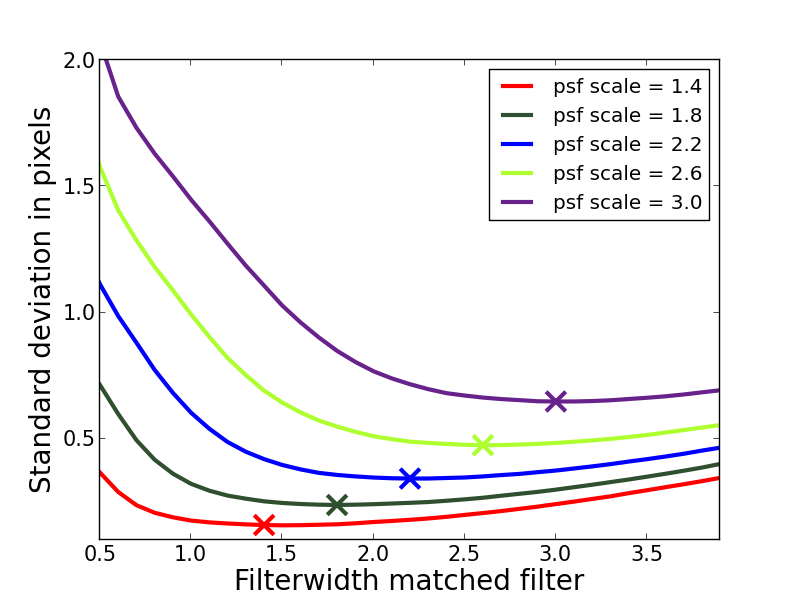
\includegraphics[width = 0.88\textwidth]{pictures/matchedFilterPlots1.png}
	 \caption{This figure shows the accuracy of detection achieved using different Gaussian filters for denoising. The cross marks the minimum of each curve.}
	\label{matchedFilter1}
\end{figure}

The figures in \ref{matchedFilter2} show the measurement, a shifted measurement curve and the result of the calculation. The measured error was larger than the calculated error, therefore the shifted line is also shown to state that the curves shape match but there is an additional error that shifts the line. \newline
These results show that the calculated standard deviation of the localization can be used to estimate the localization error of SimpleSTORM for further calculations or error propagation.

\begin{figure}
\subfloat[PSFs scale = 2.6]{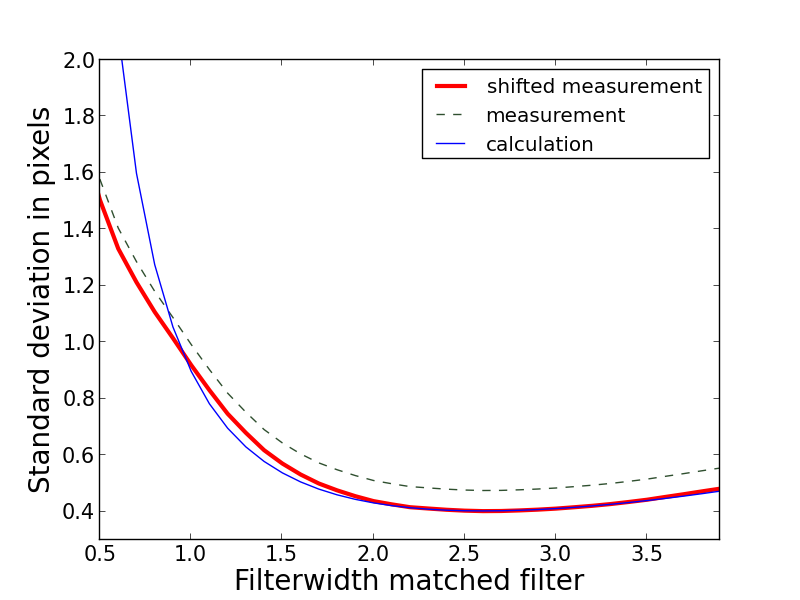
\includegraphics[width = 0.485\textwidth]{pictures/matchedFilterPlots2.png}}\hfill
\subfloat[PSFs scale = 1.8]{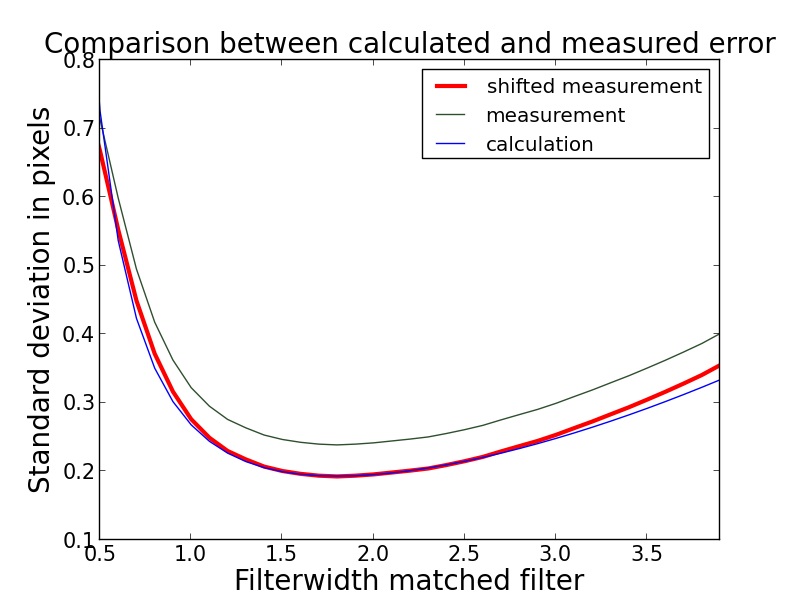
\includegraphics[width = 0.485\textwidth]{pictures/matchedFilterPlots3.png}}
	\caption{Comparison between the measured and the calculated localization error. The dashed lines show the unchanged measurement results, for better comparism the line was shifted to match the calculated error.}
	\label{matchedFilter2}	
\end{figure}

\section{Test PSF estimation}
The estimation of the width of the point spread function of the signal is very important. The localization error increases with larger deviations of the matched filters width from the true width of the PSF, as shown in \ref{detectionError}. \newline
Figure \ref{estimatedSigma} shows the results of an accuracy test. For this test, data was created artificially. One PSF was simulated at a random location with a fixed width, poisson noise was added. The signal-to-noise ratio was set to 10. Then this width was estimated by the SimpleSTORM algorithm. This was done with values for the standard deviation of the Gaussian in a range from 0.2 up to 4. The plot shows that for standard deviations up to 2.5 the estimated value for the width is very close to the actual value. The wider the PSF becomes in the spatial domain the smaller it gets in the Fourier domain. This is the reason why the accuracy of the estimation is decreasing for larger widths. This effect can be reduced by choosing a larger region of interest for the power spectrums acumulation. The parameter chosen for the plot in figure \ref{estimatedSigma} was the default value. The typical width of the PSF for real world data is in a range of 1 to 2, this is a range in which the estimation gives reliable results.\newline
\begin{figure}
\centering
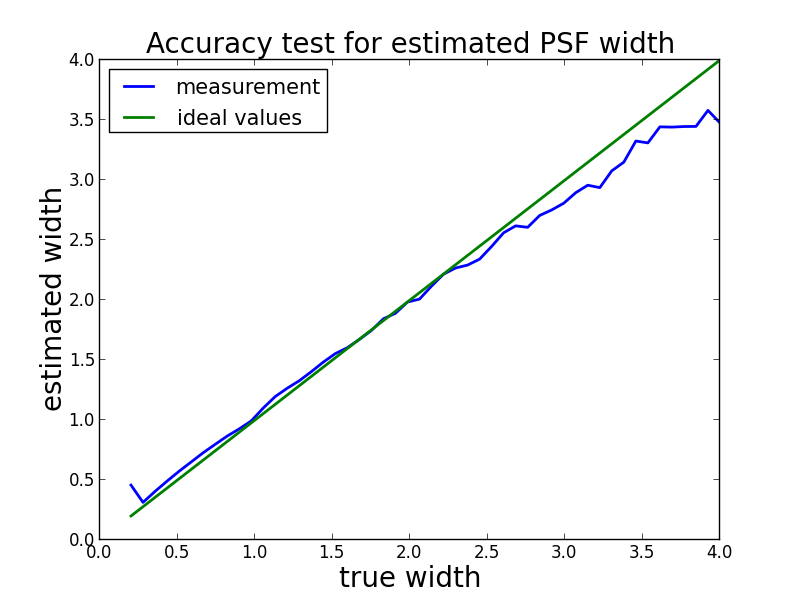
\includegraphics[width = 0.88\textwidth]{pictures/AccuracyTestPSFWidth.png}
	 \caption{The figure shows the estimated widths of the point spread function plotted over the true widht of the simulated signal. The signal-to-noise ratio was 10 for this test. The green line shows the simulated values.}
	\label{estimatedSigma}
\end{figure}


\section{Bleaching signal}
One assumption was that the backgrounds illumination is caused mainly from out of focus fluorophors and is therefore Poission distributed. If this is the case the background illumination should decrease over time. Bleaching of fluorophores describes the process in which the fluorescent molecules change their conformation and lose the ability to emit light permanently. The spectrum of the emission can also change so that the fluorescent molecules can not be detected any more. All fluorophores used for the STORM images available to us bleach over time. This decay of the mean backgrounds intensity is shown in figure \ref{bleaching}.

\begin{figure}
\centering
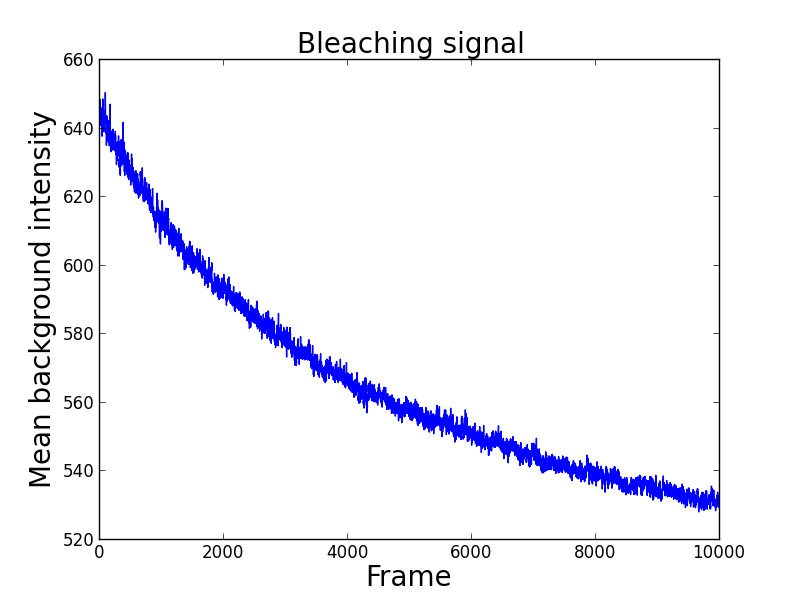
\includegraphics[width = 0.5\textwidth]{pictures/bleaching.png}
	\caption{The number of active fluorophores decreases over time and so does the mean intensity of the image. This picture shows the mean intensities of 10 background pixel over time. }
	\label{bleaching}
\end{figure}